\chapter{\textit{Grasp}について}
\label{graspについて}

\section{概要}
\ref{related_works}章では、FelsのEmbodimentを説明し、「身体化するまでの過程」から本研究の位置付けを整理し、先行研究や作品実践に対しても同じ視点から相違点の説明を試みた。
本章では、研究の主題である「時間がかかり、もどかしさを経験するような使いづらさ」を捉えるため、\textit{grasp}という概念を定義する。この\textit{grasp}という概念は、これまでに行ってきた試作とデスクリサーチから辿り着いた概念である。そのため、この概念に到達するまでに行ったプロトタイピングと、FelsのEmbodimentにまつわる議論との関連を示すことで、この概念の妥当性を補強する。その上で、\textit{grasp}についての仮説を提示する。\\

\section{\textit{grasp}の定義}
\label{grasp_difinition}
\textit{grasp}とは、\textbf{「人とオブジェクトの関係の中で、人がある対象に注意や目的意識を抱きながら、意識的に試行する期間」}であると定義する。
graspは「把握」を意味する動詞でもあるが、ここで「動作」ではなく「期間」とした。その理由は、「意識的に試行する」とき、同時にその結果を受けて気づきを得たり、その気づきをもとに新たな関心を抱くといった、単に自分が行為しているだけではなく、対象から影響を受けながら次の行為が決まってくるようなフィードバックループの構造があると考えるためである。「grasp=把握」という言葉についても、単に「ものを掴む」という意味だけでなく、「理解」の意味があることは、対象について一方向に働きかけているのではない様子が現れているのではないだろうか。

\textit{grasp}とは例えば、ギターの習得過程において、弾きこなしたいフレーズを定め、それを達成するまでに試行錯誤をし、達成できるようになるまでの期間である。熟達した状態では、熟達する前とは違う視座でものごとを捉えられるようになり、また違う対象に注意が向くようになると、ギターと人との間に別の\textit{grasp}が芽生える。
またあるいは、\textit{grasp}の過程で、対象と向き合い続ける過程の中でその解像度が高まり、当初目指していたこととは違うことに興味を抱く(セレンディピティ)ことでも、別の\textit{grasp}が芽生える。

ここまで具体例を通してみてきたように、\textit{grasp}は、ギターと人との関係において一度だけ生じるのではなく、注目する対象が定まれば何度でも生じる。
% ここで、\textit{grasp}は人とオブジェクトの関係の中で、人が注意を向ける「対象」ごとに別の\textit{grasp}があると言えそうだが、注意を向けている「対象」がなんであるか、断言できなかったり、本人も判然としないこともある。そのため、

\section{Felsの議論との関係性}
ここでは\textit{grasp}が、FelsのEmbodimentとどう関係するのかについて説明する。
先の節\ref{grasp_difinition}に挙げたように、人は\textit{grasp}を通して、あるいはその過程で、オブジェクトから影響を受けながら次の試行が形作られていく。この時の「試行」には、挙動を確かめるような動作、すなわちFelsの「Response」もあれば、試行を通して得られた結果をもとに、何かに考えを巡らす「Contemplation」も含まれる。こうした試行の積み重なりから、人とオブジェクトのあいだに「Control」や「Belonging」の関係、すなわちFelsの意味でのEmbodimentが生じるのではないか。

つまりこの概念は、試行することと一体化することの「間」に行われていることについて語ることを可能にするものである。\textit{grasp}の様相を捉えることで、現状からEmbodimentが達成されるまでのあいだに欠けているものが何であるかを語る術を得られるのではないか、と考える。

\section{\textit{grasp}に辿り着くまでのプロトタイピング}
\label{prototyping_concept_making}
作品のもととなった試行は当初、「動きのスケッチツール」というまったく別の目的で作られたシステムである。\\
ピアノを弾く時のように、人は10本ある指を同時に操り、その組み合わせから柔軟で緻密な動作を作ることができる。手のストロークを記録し、静止画をスケッチする場として「紙とペン」があるように、手の動きをそのまま記録し、「動きをスケッチする」場として新しいインターフェースを設計することを案じていた。\\
しかし手指は人間の身体の中でもとりわけ随意に動かすことのできる器官である。だからこそ、動きを入力するためのインターフェースは、手と異なる形状であったとしても自在に操ることができるのではないか。もしそうであるならば、人間の身体構造による制約を超えた「動きのスケッチ」が達成できる、と考えた。\\
そうして、手指の動きをトラッキングしつつ、画面上でその動きは別の形へマッピングされて動くインターフェースを制作し、IAMAS Open House 2022にて展示した。この時点では、動きを記録する機能は存在しておらず、あくまで手と、それに伴って動く手指とは異なる形の動きが確認できるだけのものであった。\\

\begin{figure}[H]
  \centering
  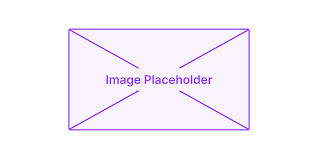
\includegraphics[width=15cm]{img/placeholder.png}
  \caption{IAMAS Open House 2022での展示のようす(2022年)}
  \label{fig:exhibit_2022}
\end{figure}

しかし実際に展示を行うと、「身体の変換」を扱った表現については、当初想定していなかった仕方で受容されることがわかった。まず1つ目に、構造としては単に手の指の動きが、別の構造にマッピングされただけであるのに、別の構造の手を動かす感覚はそれだけで「快」がある体験だということである。その「快」の正体はこの時点ではわからなかったが、手指の変換が3パターン展示された状態のこの展示で、10分以上興味を持って体験する方が複数名いた。またもう1つに、制作されたプロトタイプを展示した際、指先を動かすだけでなく、カメラに対して手を近づけたり遠ざけたり、手を裏返したりするなど、さまざまな体験の方法が現れたことに興味を持った。これは、手指の動きが別の形状にマッピングされたことで、「反応している」ということは分かっていても「どのように反応しているのか」についてははっきりせず、それを確かめるように身体を動かしているのだと考えた。変換方法を実装した制作者は仕組みを知ってしまっているので、こうした試行は起こり得ないが、どのように変換されているのかを知り得ない体験者は、自身の体を動かして観察されたことでのみ、その動作原理を推測することになるので、最初にどう身体を動かしたかによって、動作原理をどう認識するかに違いが現れるのではないかと考えた。これをきっかけとして、手指の運動を用いた表現について「動きのスケッチツール」というテーマから離れ、「手指の変換表現」について幅広く検討する中で、こうした興味を掘り下げていくことにした。

「快」の正体に迫る上で、仮説として「手指特有の動きに対する美的関心(動きに対する快)」、「手指を動かすことに対する快(身体動作における快)」が挙げられる。\\
そこで、インタラクションのあるものについての発散と、インタラクションのないモーショングラフィックについての発散を行なった。それを踏まえて、インタラクションのあるものについての発散を試みた。


\section{\textit{grasp}の性質}
\textit{grasp}には二つの性質がある。一つは、時間幅が注意を向けている対象によって、長い場合と短い場合があることである。目的意識が芽生えてからスムーズに操作できるようになる場合、'reach'から'manipulate'が近く、\textit{grasp}は短い、すなわち直感的で使いやすいものとして経験される。その一方、目的意識が芽生えてから試行錯誤を伴い、習熟に長い期間を要する場合、\textit{grasp}は長く、もどかしさを経験し、操れるようになった時に達成感を経験する。\\

二つ目に、\textit{grasp}の過程で他のことに対する意識が次々と芽生えることがある。具体的には「やってみるまでわからない」といった経験や、物事に対する解像度が高まる中で、当初とは異なる意識が芽生える状況に相当する。\\

このコンセプトを展開し、「試行錯誤の余地」を設計することを目指したのが、修士作品《Grasp(er)》である。この作品では、\textit{grasp}を経験する中で、個人による創造的な活動が生まれ、\textit{grasp}という動作を行っているのではなく、そこに'er'の接尾辞がついた'Grasper'であると名付けた。